\chapter{深入集合Collection}
课前思考:
\begin{enumerate}
	\item Java中有哪些常用集合类?
	\item Java常用集合类如何实现的?
	\item 不同集合类在什么场合下使用?
	\item 不同集合类其性能如何?
\end{enumerate}
\section{集合框架与ArrayList}
\subsection{Java集合框架}
\begin{figure}[!h]
	\centering
	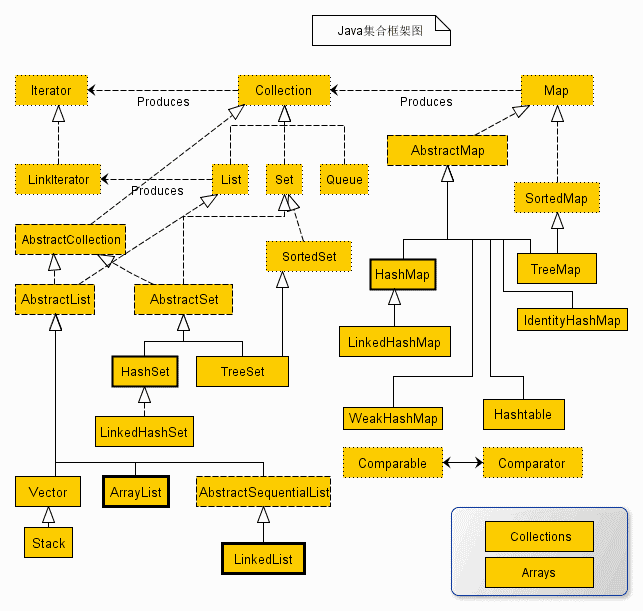
\includegraphics[width=\textwidth]{image/collection.png}
	\caption{Java集合框架图}
\end{figure}
\subsection{常用集合类}
\begin{itemize}
	\item List
	\subitem ArrayList
	\subitem LinkedList
	\item Map
	\subitem HashMap
	\subitem HashTable
	\subitem TreeMap
	\subitem LinkedHashMap
	\item Set
	\subitem HashSet
	\subitem TreeSet
	\subitem LinkedHashSet
\end{itemize}
\subsection{ArrayList}
\begin{itemize}
	\item List接口的可变数组的实现。实现了所有可选列表操作,并允许null在内的所有元素。
	\item 非线程安全
	\item 底层使用的数据结构为数组
	\item 适合查改,弱于增删
\end{itemize}
\subsection{ArrayList实现分析}
\noindent 1. 用指定的元素替代此列表中指定位置上的元素,并返回以前位于该位置上的元素。
\begin{lstlisting}[language=java]
public E set(int index, E element) {
	rangeCheck(index);
	
	E oldValue = elementData(index);
	elementData[index] = element;
	return oldValue;
}
\end{lstlisting}
2. 将指定的元素添加到此列表的尾部。
\begin{lstlisting}[language=java]
public boolean add(E e) {
	ensureCapacityInternal(size + 1);  // Increments modCount!!
	elementData[size++] = e;
	return true;
}
\end{lstlisting}
3. 将指定的元素插入此列表中的指定位置。如果当前位置有元素,则向右移动当前位于该位置
的元素以及所有后续元素(将其索引加1),设计数组拷贝,插入速度不及add(E element)方法。
\begin{lstlisting}[language=java]
public void add(int index, E element) {
	rangeCheckForAdd(index);
	
	ensureCapacityInternal(size + 1);  // Increments modCount!!
	System.arraycopy(elementData, index, elementData, index + 1,
	size - index);
	elementData[index] = element;
	size++;
}
\end{lstlisting}
4. 移除此列表中指定位置上的元素。涉及数组拷贝。
\begin{lstlisting}[language=java]
public E remove(int index) {
	rangeCheck(index);
	
	modCount++;
	E oldValue = elementData(index);
	
	int numMoved = size - index - 1;
	if (numMoved > 0)
		System.arraycopy(elementData, index+1, elementData, index, numMoved);
	elementData[--size] = null; // clear to let GC do its work
	
	return oldValue;
}
\end{lstlisting}
5. 数组扩容,按照1.5倍方式扩容。涉及数组拷贝、速度慢。
\begin{lstlisting}[language=java]
public void ensureCapacity(int minCapacity) {
	//private static final Object[] DEFAULTCAPACITY_EMPTY_ELEMENTDATA = {};
	//private static final int DEFAULT_CAPACITY = 10;
	int minExpand = (elementData != DEFAULTCAPACITY_EMPTY_ELEMENTDATA)
		// any size if not default element table
		? 0
		// larger than default for default empty table. It's already
		// supposed to be at default size.
		: DEFAULT_CAPACITY;
	
	if (minCapacity > minExpand) {
		ensureExplicitCapacity(minCapacity);
	}
}

private void ensureExplicitCapacity(int minCapacity) {
	modCount++;
	
	// overflow-conscious code
	if (minCapacity - elementData.length > 0)
		grow(minCapacity);
}

private void grow(int minCapacity) {
// overflow-conscious code
// private static final int MAX_ARRAY_SIZE = Integer.MAX_VALUE - 8;
	int oldCapacity = elementData.length;
	int newCapacity = oldCapacity + (oldCapacity >> 1);
	if (newCapacity - minCapacity < 0)
		newCapacity = minCapacity;
	if (newCapacity - MAX_ARRAY_SIZE > 0)
		newCapacity = hugeCapacity(minCapacity);
	// minCapacity is usually close to size, so this is a win:
	elementData = Arrays.copyOf(elementData, newCapacity);
}

private static int hugeCapacity(int minCapacity) {
	if (minCapacity < 0) // overflow
		throw new OutOfMemoryError();
	return (minCapacity > MAX_ARRAY_SIZE) ?
		Integer.MAX_VALUE :
		MAX_ARRAY_SIZE;
}
\end{lstlisting}

\section{LinkedList}
\begin{itemize}
	\item List接口的链接列表实现,实现所有的列表操作,并且允许所有元素(包括null)
	\item 实现了Deque接口,为add、poll提供先进先出队列操作以及其他堆栈和双端队列操作。
	\item 非线程安全
	\item 适合增删,弱于查改。
\end{itemize}
1. 基于节点Node实现:(还有基于Entry)
\begin{lstlisting}[language=java]
private static class Node<E> {
	E item;
	Node<E> next;
	Node<E> prev;
	
	Node(Node<E> prev, E element, Node<E> next) {
		this.item = element;
		this.next = next;
		this.prev = prev;
	}
}
\end{lstlisting}
2. 根据序号获取Node对象
\begin{lstlisting}[language=java]
public E get(int index) {
	checkElementIndex(index);
	return node(index).item;
}

private void checkElementIndex(int index) {
	if (!isElementIndex(index))
	throw new IndexOutOfBoundsException(outOfBoundsMsg(index));
}

private boolean isElementIndex(int index) {
	return index >= 0 && index < size;
}

Node<E> node(int index) {
	// assert isElementIndex(index);
	
	if (index < (size >> 1)) {
		Node<E> x = first;
		for (int i = 0; i < index; i++)
			x = x.next;
		return x;
	} else {
		Node<E> x = last;
		for (int i = size - 1; i > index; i--)
			x = x.prev;
		return x;
	}
}
\end{lstlisting}
3. 在某一个节点前添加元素
\begin{lstlisting}[language=java]
void linkBefore(E e, Node<E> succ) {
	// assert succ != null;
	final Node<E> pred = succ.prev;
	final Node<E> newNode = new Node<>(pred, e, succ);
	succ.prev = newNode;
	if (pred == null)
		first = newNode;
	else
		pred.next = newNode;
	size++;
	modCount++;
}
\end{lstlisting}
4. 指定位置添加元素,需要先找到index的元素,然后添加。
\begin{lstlisting}[language=java]
public void add(int index, E element) {
	checkPositionIndex(index);
	
	if (index == size)
		linkLast(element);
	else
		linkBefore(element, node(index));
}
\end{lstlisting}
5. 队首队尾添加元素
\begin{lstlisting}[language=java]
//队首插入元素
public void addFirst(E e) {
	linkFirst(e);
}
private void linkFirst(E e) {
	final Node<E> f = first;
	final Node<E> newNode = new Node<>(null, e, f);
	first = newNode;
	if (f == null)
		last = newNode;
	else
		f.prev = newNode;
	size++;
	modCount++;
}

public void addLast(E e) {
	linkLast(e);
}
//队尾添加元素
void linkLast(E e) {
	final Node<E> l = last;
	final Node<E> newNode = new Node<>(l, e, null);
	last = newNode;
	if (l == null)
		first = newNode;
	else
		l.next = newNode;
	size++;
	modCount++;
}
\end{lstlisting}
6. 删除元素
\begin{lstlisting}[language=java]
public boolean remove(Object o) {
	if (o == null) {
		for (Node<E> x = first; x != null; x = x.next) {
			if (x.item == null) {
				unlink(x);
				return true;
			}
		}
	} else {
		for (Node<E> x = first; x != null; x = x.next) {
			if (o.equals(x.item)) {
				unlink(x);
				return true;
			}
		}
	}
	return false;
}
\end{lstlisting}
实际操作:
\begin{lstlisting}[language=java]
E unlink(Node<E> x) {
	// assert x != null;
	final E element = x.item;
	final Node<E> next = x.next;
	final Node<E> prev = x.prev;
	
	if (prev == null) {
		first = next;
	} else {
		prev.next = next;
		x.prev = null;
	}
	
	if (next == null) {
		last = prev;
	} else {
		next.prev = prev;
		x.next = null;
	}
	
	x.item = null;
	size--;
	modCount++;
	return element;
}
\end{lstlisting}
其他删除操作:
\begin{lstlisting}[language=java]
public E removeFirst() {
	final Node<E> f = first;
	if (f == null)
		throw new NoSuchElementException();
	return unlinkFirst(f);
}

public E removeLast() {
	final Node<E> l = last;
	if (l == null)
		throw new NoSuchElementException();
	return unlinkLast(l);
}

public E remove(int index) {
	checkElementIndex(index);
	return unlink(node(index));
}
\end{lstlisting}
\subsection{List的适用范围}
\begin{itemize}
	\item ArrayList适用于对于数据查询修改大于数据增删的场合;
	\item LinkedList适用于对于数据增删大于数据查询的场合。
\end{itemize}

\section{HashMap和HashTable}
\subsection{HashMap}
\begin{itemize}
	\item 基于哈希表的Map接口实现,提供所有可选的映射操作,并允许使用null值和null键。
	\item 非线程安全
	\item 不保证映射的顺序,特别是不保证该顺序恒久不变。
\end{itemize}
\subsection{HashMap数据结构}
\begin{lstlisting}[language=java]
transient Node<K,V>[] table;
static class Node<K,V> implements Map.Entry<K,V> {
	final int hash;
	final K key;
	V value;
	Node<K,V> next;
	
	Node(int hash, K key, V value, Node<K,V> next) {
	this.hash = hash;
	this.key = key;
	this.value = value;
	this.next = next;
	//......
}
\end{lstlisting}
\subsection{HashMap实现分析}
\begin{lstlisting}[language=java]
public V put(K key, V value) {
	return putVal(hash(key), key, value, false, true);
}
final V putVal(int hash, K key, V value, boolean onlyIfAbsent,
boolean evict) {
	Node<K,V>[] tab; Node<K,V> p; int n, i;
	if ((tab = table) == null || (n = tab.length) == 0)
		n = (tab = resize()).length;
	if ((p = tab[i = (n - 1) & hash]) == null)
		tab[i] = newNode(hash, key, value, null);
	else {
		Node<K,V> e; K k;
		if (p.hash == hash &&
				((k = p.key) == key || (key != null && key.equals(k))))
			e = p;
		else if (p instanceof TreeNode)
			e = ((TreeNode<K,V>)p).putTreeVal(this, tab, hash, key, value);
		else {
			for (int binCount = 0; ; ++binCount) {
				if ((e = p.next) == null) {
					p.next = newNode(hash, key, value, null);
					if (binCount >= TREEIFY_THRESHOLD - 1) // -1 for 1st
						treeifyBin(tab, hash);
					break;
				}
				if (e.hash == hash &&
					((k = e.key) == key || (key != null && key.equals(k))))
					break;
				p = e;
			}
		}
		if (e != null) { // existing mapping for key
			V oldValue = e.value;
		if (!onlyIfAbsent || oldValue == null)
			e.value = value;
		afterNodeAccess(e);
		return oldValue;
		}
	}
	++modCount;
	if (++size > threshold)
		resize();
	afterNodeInsertion(evict);
	return null;
}

static final int hash(Object key) {
	int h;
	return (key == null) ? 0 : (h = key.hashCode()) ^ (h >>> 16);
}
\end{lstlisting}
\begin{lstlisting}[language=java]
public V get(Object key) {
	Node<K,V> e;
	return (e = getNode(hash(key), key)) == null ? null : e.value;
}

final Node<K,V> getNode(int hash, Object key) {
	Node<K,V>[] tab; Node<K,V> first, e; int n; K k;
	if ((tab = table) != null && (n = tab.length) > 0 &&
		(first = tab[(n - 1) & hash]) != null) {
		if (first.hash == hash && // always check first node
			((k = first.key) == key || (key != null && key.equals(k))))
			return first;
		if ((e = first.next) != null) {
			if (first instanceof TreeNode)
				return ((TreeNode<K,V>)first).getTreeNode(hash, key);
			do {
				if (e.hash == hash &&
				((k = e.key) == key || (key != null && key.equals(k))))
					return e;
			} while ((e = e.next) != null);
		}
	}
	return null;
}
\end{lstlisting}
\subsection{HashTable的特点}
\begin{itemize}
	\item HashTable和HashMap采用相同的存储机制,二者的实现基本一致;
	\item 不允许有null值的存在;
	\item HashTable是线程安全的,内部实现基本都是synchronized。
	\item 迭代器具有强一致性。
\end{itemize}

\section{TreeMap与LinkedHashMap}
\subsection{TreeMap}
\begin{itemize}
	\item Map接口的树实现;
	\item 不允许null值的存在;
	\item 非线程安全;
	\item 键值有序;
	\item 使用了红黑树,O(log n)查找时间复杂度。
\end{itemize}
\subsection{TreeMap实现分析}
\begin{itemize}
	\item Entry是红黑树的节点,包含了红黑树的6个基本组成部分:\textbf{key、value、left、right、parent、color}。Entry节点根据key排序,Entry点包含的内容为value。
	\item 红黑树排序时,根据Entry中的key进行排序。Entry的key比较大小是根据比较器comparator来进行判断的。
\end{itemize}
\subsection{TreeMap的优势}
\begin{enumerate}
	\item 空间利用率高
	\subitem HashMap的数组大小必须为2的n次方;
	\subitem TreeMap中树的没一个节点就代表了一个元素;
	\item 性能稳定
	\subitem Hash碰撞会导致HashMap查询开销提高;
	\subitem HashMap扩容时会rehash,开销高;
	\subitem TreeMap的操作均能在O(log n)内完成。
\end{enumerate}
\subsection{LinkedHashMap}
\begin{itemize}
	\item Map接口的哈希表和链接列表实现,提供所有可选的映射操作,并允许使用null值和null键
	\item 非线程安全
	\item 具有可预知的迭代顺序
\end{itemize}
\subsection{LinkedHashMap实现}
\begin{lstlisting}[language=java]
Node<K,V> newNode(int hash, K key, V value, Node<K,V> e) {
	LinkedHashMap.Entry<K,V> p =
		new LinkedHashMap.Entry<K,V>(hash, key, value, e);
	linkNodeLast(p);
	return p;
}
public V get(Object key) {
	Node<K,V> e;
	if ((e = getNode(hash(key), key)) == null)
		return null;
	if (accessOrder)
		afterNodeAccess(e);
	return e.value;
}
\end{lstlisting}
\subsection{Map的适用范围}
\begin{itemize}
	\item HashMap适用于一般的键值映射需求;
	\item HashTable适用于有多线程并发的场合;
	\item TreeMap适用于要按照键排序的迭代场合;
	\item LinkedHashMap适用于特殊顺序的迭代场合(如LRU算法)。
\end{itemize}

\section{HashSet}
\begin{itemize}
	\item 实现Set接口,由哈希表支持,允许使用null元素;
	\item 非线程安全;
	\item 不保证set的迭代顺序,特别是不保证该顺序恒久不变
\end{itemize}
\begin{lstlisting}[language=java]
//底层使用HashMap保存HashSet所有元素
private transient HashMap<E,Object> map;
//定义一个虚拟的Object对象作为HashMap的Value
private static final Object PRESENT = new Object();
//借助HashMap的add添加,HashMap的add方法可以返回该key之前的value,如果为null则说明之前尚未添加,即HashSet可以添加该元素
public boolean add(E e) {
	return map.put(e, PRESENT)==null;
}
//借助HashMap的方法来查找
public boolean contains(Object o) {
	return map.containsKey(o);
}
\end{lstlisting}
\subsection{Set的特点}
\begin{itemize}
	\item HashSet通过HashMap实现,TreeSet通过TreeMap实现,LinkedHashSet通过LinkedHashMap实现,
	Set类与Map类拥有近似的使用特性。
\end{itemize}